\documentclass
% [landscape]
{article}

\usepackage{ctex}
\usepackage{amsmath}
\usepackage{graphicx}
\usepackage{epstopdf}
\usepackage{tikz}
\usepackage{psfrag}
\usepackage{natbib}
\usepackage{hyperref}

\begin{document}

\renewcommand{\refname}{参考文献}
\renewcommand{\figurename}{图}
\renewcommand{\abstractname}{摘要}

\title{磁流体力学数值模拟方法第1次作业}


\author{赵世娟\footnote{Email:sjzhao2025@mail.ustc.edu.cn}\\SA25007037
  \and
  温雨鑫\footnote{Email:}\\SA25007032
\and
 杨宇锋\footnote{Email:}\\SA25007034
}

\date{%
\scriptsize%
% CAS Key Laboratory for Basic Plasma Physics, School of Earth and Space Sciences,
% \\
% University of Science and Technology of China, Hefei, Anhui 230026, China
% \\
中国科学技术大学地球与空间科学学院, 合肥 230026
%
}

\maketitle

\begin{abstract}
本次作业我们学习了磁流体力学波的相速度、磁化等离子体中的色散关系、磁流体力学快磁声激波关系的原理，用Python进行了编程成图，并对它们
进行了分析讨论，最后用LATEX编写了文档。
\end{abstract}

\section{引言}
等离子体是由离子、电子和中性粒子组成的导电气体，作为物质存在的第四态，
占据了宇宙物质的 99.9\% 以上\citep{Diver2001}。从恒星内部、星际介质到
行星磁层、电离层，等离子体广泛存在于各种天体物理和空间环境中。
深入研究等离子体的动力学行为，对于理解空间物理现象、探索天体物理过程
以及推动实验室等离子体应用都具有重要的科学价值。

在研究空间等离子体的过程中，根据不同的时空尺度和物理条件，
研究者们发展了多种理论模型来描述等离子体的行为。
磁流体力学（Magnetohydrodynamics, MHD）是将等离子体视为导电流体，
结合流体力学方程和麦克斯韦方程组而建立的宏观理论框架\cite {Jeffrey1964}。
这种近似适用于研究大尺度、低频的等离子体现象，能够有效描述等离子体
与磁场的相互作用过程。在MHD理论框架下，可以研究各种等离子体波的
传播特性，包括阿尔芬波、快慢磁声波等基本波模。

冷等离子体近似是另一种重要的理论模型，它忽略粒子的热运动效应，
主要考虑带电粒子在磁场中的回旋运动。在此近似下，可以得到等离子体
的色散关系，描述波的频率与波矢之间的关系\citep{Diver2001}。
冷等离子体理论可以解释许多空间和实验室等离子体中观测到的波现象，
如哨声波、离子回旋波等。

激波是等离子体中另一种重要的非线性现象。当波的振幅足够大时，
非线性效应将导致波形发生畸变，形成激波。磁流体力学激波在太阳风
与行星磁层的相互作用、日冕物质抛射等空间物理过程中扮演着重要角色\citep{Jeffrey1964}。

本文主要研究以下三个方面的内容：（1）磁流体力学波的相速度特性，
分析快慢磁声波和阿尔芬波在不同参数下的传播特征；（2）磁化冷等离子体
的色散关系，研究不同传播方向和频率范围内的波模；（3）磁流体力学
快磁声激波关系，分析激波的参数依赖特性。



\section{磁流体力学波的相速度图}
\subsection{原理和基本公式}

磁流体力学中, 快慢磁声波, 横波 (Alfven) 的特征速度分别为\citep{Jeffrey1964}
\begin{align}
c_f &= \left\{\frac{1}{2} \left[a^2 + b^2 + \sqrt{(a^2 + b^2)^2 - 4 a^2 b^2
\cos^2\theta}\right]\right\}^{1/2} 
\end{align}
\begin{align}
c_s &= \left\{\frac{1}{2} \left[a^2 + b^2 - \sqrt{(a^2 + b^2)^2 - 4 a^2 b^2
\cos^2\theta}\right]\right\}^{1/2}, 
\\
b_n &= b \left|\cos\theta\right|
\end{align}
其中, $a$ 是声速, $a^2 = \frac{\partial p}{\partial \rho}$, $p$ 和 $\rho$ 是流体的压力和密度;
$b$ 是 Alfven 波速, $b^2 = \frac{\mu H^2}{4 \pi \rho}$. $\boldsymbol{H}$ 是磁场, $\mu$ 是磁导率;
$\theta$ 为传播方向和磁场所成夹角.
\subsection{实现及结果讨论}
我们将上述的将以上公式中 $c_f$, $c_s$进行无量纲化处理，然后在极坐标中将 $\frac{c_f}{b}$, $\frac{c_s}{b}$和 $\theta$ 的关系用图形表示了出来。
\begin{align}
\frac{c_f}{b} &=\left\{\frac{1}{2}\left[s^2+1+\sqrt{(s^2+1)^2-4 s^2 cos^2\theta}\right]\right\}^{1/2}
\\
\frac{c_s}{b} &=\left\{\frac{1}{2}\left[s^2+1-\sqrt{(s^2+1)^2-4 s^2 cos^2\theta}\right]\right\}^{1/2}
\\
\frac{b_n}{b} &=\left|\cos \theta\right| 
\end{align}
其中$ s=\frac{a^2}{b^2}$
% \begin{figure}[h]
% \begin{minipage}[t]{1.0\linewidth}
% \centering
% %\begin{center}
% 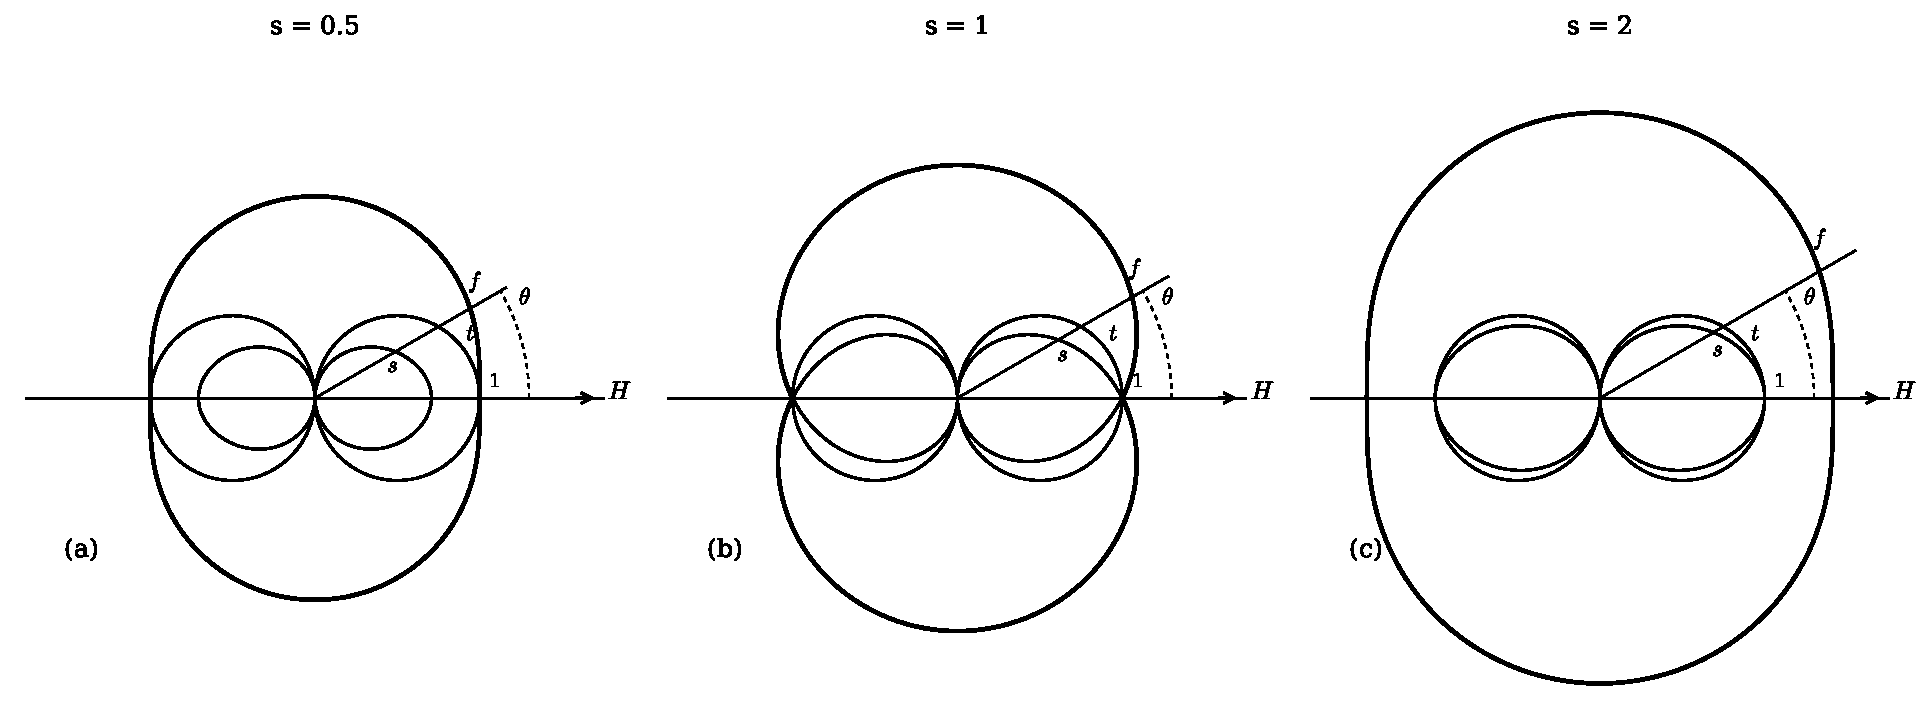
\includegraphics[width=1\textwidth]{Friedrich.pdf}
% \caption{磁流体力学波的相速度图 (a) $s = 0.5$, (b) $s=1$, (c) $s=2$.}\label{Friedrich}
%  %\end{center}
%  \end{minipage}
% \end{figure}
\par 从图~\ref{Friedrich}中可以看出，任何时候都有$c_s \le c_a \le c_f $
\begin{itemize}
\item 当声速小于阿尔芬速度时，在于磁场平行的方向上，阿尔芬速度等于快磁声波的速度.
\item 当声速等于阿尔芬速度时，在于磁场平行的方向上，慢磁声波速度、阿尔芬速度与快磁声波的速度均相等.
\item 当声速大于阿尔芬速度时，在于磁场平行的方向上，阿尔芬速度等于慢磁声波的速度.
\end{itemize}
\section{冷等离子体中的色散关系}



\subsection{原理和基本公式}
磁化冷等离子体的色散关系可以表示为\citep{Diver2001}
\begin{align}
\left(S \sin^2 \theta + P \cos^2 \theta\right) n^4 - \left[R L \sin^2 \theta
+ P S \left(1 + \cos^2 \theta\right) \right] n^2 + P R L= 0 \label{Eqn:Colp}
\end{align}
这里 $n = k c / \omega$ 是折射率, $\theta$ 是波的传播方向和磁场的夹角,
\begin{align*}
S & = (R + L) / 2
\\
D &= (R - L) / 2
\\
R &= 1 - \sum_s \frac{\omega_{ps}^2}{\omega^2} \frac{\omega}{\omega + \omega_{cs}}
\\
L &= 1 - \sum_s \frac{\omega_{ps}^2}{\omega^2} \frac{\omega}{\omega - \omega_{cs}}
\\
P &= 1 - \sum_s \frac{\omega_{ps}^2}{\omega^2}  = 1 - \frac{\omega_p^2}{\omega^2}
\end{align*}
其中 $\omega_{ps}$ 和 $\omega_{cs}$ 分别是第 $s$ 种类粒子的等离子体频率和回旋频率, $\omega_p$ 是整体的等离子体频率. 方程(\ref{Eqn:Colp}) 还可以写成如下的形式,
\begin{align}
\tan^2 \theta &= - \frac{P (n^2 - R) (n^2 - L)}{(S n^2 - R L) (n^2 - P)}.
\end{align}
\subsection{实现及结果讨论}
\par 冷等离子体单成分的结果见图~\ref{ColdPlasma}.从图中可以看到，冷等离子体中主要存在如下几种波：
\par （1）平行传播 
\begin{itemize}
\item 等离子体振荡(Plasma Oscillations): $\theta=0 \rightarrow P=0$ and $\omega^2=\omega^{2}_{p}$. 这是一种静电等离子体振荡，静电场平行于背景磁场.
\item 圆极化波(Circularly polarized waves):$\theta=0 \rightarrow n^2=R$  (右旋)and $ n^2=L$(左旋).
\end{itemize}

% \begin{figure}[h]
% \begin{minipage}[t]{1.0\linewidth}
% \centering
% %\begin{center}
% %\begin{tabular}{cc}
% \includegraphics[width=0.9\textwidth]{coldp.pdf} 
% %\end{tabular}
% \caption{磁化冷等离子体的色散关系.  $\omega_p / \omega_c = 0.5$ 和 $\omega_p / \omega_c = 2$} \label{ColdPlasma}
% %\end{center}
% \end{minipage}
% \end{figure}

\par （2）共振和截止(Resonances and Cut-Offs)-平行传播
\begin{itemize}
\item 阿尔芬波(Alfven Wave):对于$\omega \ll \omega_{ci}$的极低频波，可以有如下近似关系
$$R \approx L \approx 1+c^{2} / c_{a}^{2}$$
进而有阿尔芬波的色散关系
$$\omega^{2} \approx \frac{k^{2} c^{2}}{1+c^{2} / c_{a}^{2}} \approx k^{2} c_{a}^{2}$$
\item 离子回旋波(Ion Cyclotron Wave):当波的频率从低频接近离子频率时，色散关系可近似表示为
$$\omega^{2} \approx \frac{k^{2} c^{2}}{2 \omega_{p i}^{2}}\left(\omega_{c i}^{2}-\omega^{2}\right)$$
\item 哨声波(whistler waves):当扰动的频率介于离子和电子回旋频率之间时，将激发哨声模，色散关系近似表示为
$$\omega^{2} \approx \frac{k^{2} c^{2}}{1+\omega_{p}^{2} /\left(\omega \omega_{c e}\right)}$$
\item 电子回旋波(Electron Cyclotron Wave):对于右旋波模，电子回旋波的色散关系近似表示为
$$n^{2} \approx 1-\frac{\omega_{p e}^{2}}{\omega\left(\omega+\omega_{c e} \cos \theta\right)}$$
\end{itemize}
\par （3）垂直传播:$\theta=\pi/2 \rightarrow n^2=P$（O模） 和 $n^2=\frac{RL}{S}$（X模）. 
\par （4）共振和截止(Resonances and Cut-Offs)-垂直传播:当S=0时，X模将表现为混杂波
$$\begin{array}{ll}
\displaystyle \omega_{u}^{2} \approx \omega_{p}^{2}+\omega_{c e}^{2}  \text { 上混杂 } \\
\displaystyle  \omega_{l}^{2} \approx \frac{\omega_{p}^{2} \omega_{c e} \omega_{c i}}{\omega_{p}^{2}+\omega_{c e}^{2}}  \text { 下混杂 }
\end{array}$$
\par （5）快阿尔芬波(Fast Alfven Wave):当极低频扰动$\omega\ll \omega_{ci}$沿垂直于磁场传播时，只有X模是可能的，近似的色散关系是
$$\omega^{2} \approx \frac{k^{2} c^{2}}{1+c^{2} / c_{a}^{2}} \approx k^{2} c_{a}^{2}$$


\section{磁流体力学快磁声激波关系}
\subsection{原理和基本公式}

磁流体力学快磁声激波关系中\citep{Jeffrey1964}, 用磁场增量 $h_f$ ($h_f \ge 0$)
来表示激波的强度, 通常分析下面的公式
\begin{align}
\frac{X_f^\pm}{h_f} = (B \pm \sqrt{R_X})/C \qquad (\ge 0) \label{Eqn:fShock}
\end{align}
和 $h_f$ 的函数关系. $B$, $C$, 和 $R_X$ 由以下表达式给出,
\begin{align}
B &= (\gamma/2) h_f \sin\theta_0 - (1-s_0),
\\
C &= 2 \sin\theta_0 - (\gamma-1) h_f,
\\
R_X &= B^2 + C(h_f + 2 s_0 \sin\theta_0) \qquad (\ge 0).
\end{align}

其中 $\theta_0$ 为波传播方向和磁场方向的夹角 ($0^\circ \le \theta_0 \le 90^\circ$),
$\gamma=5/3$ 是多方指数. 讨论两种情况, 即 $B$ 在 $C$ 的零点
\begin{align*}
\hat{B} \equiv B(\hat{h}_f) = \frac{\gamma}{\gamma-1} \sin^2\theta_0 - (1-s_0),
\end{align*}
大于等于和小于零的情况, 此处 $\hat{h}_f$ 是 $C=0$ 的根
\begin{align}
\hat{h}_f = \left(\frac{2}{\gamma-1}\right) \sin\theta_0.
\end{align}
具体表现为 $s_0$ 的条件
\begin{align}
s_0 \ge 1 - \gamma \frac{\sin^2\theta_0}{(\gamma-1)},
\end{align}
和
\begin{align}
s_0 < 1 - \gamma \frac{\sin^2\theta_0}{(\gamma-1)}.
\end{align}
而 $\hat{\hat{h}}_f$ 是 $R_X = 0$ 的根,
\begin{align}
& \hat{\hat{h}}_f = \frac{1}{2(\gamma-1) - \frac{1}{2} \gamma^2 \sin^2
\theta_0}\Big\{\sin\theta_0
(2-\gamma)(1+s_0) \nonumber
\\
& \quad + 2\cos\theta_0 \sqrt{(\gamma-1)(1-s_0)^2 + s_0 \gamma^2 \sin^2\theta_0}\Big\}.
\end{align}
将关系~(\ref{Eqn:fShock}) 用图形表示 (取 $\theta_0=15^\circ$,$s_{0}=1/2$),
形成图~\ref{FShock}，更进一步的信息可参考文献 \citep[ 229 页]{Jeffrey1964}.

\subsection{实现及结果讨论}

由图 \ref{FShock} 可知，快磁声激波存在两种类型：1 型激波（实线）和 2 型激波（虚线），
分别对应条件 $s_0 > 1 - \gamma\frac{\sin^2\theta_0}{\gamma  -1}$ 
和 $s_0 < 1 - \gamma\frac{\sin^2\theta_0}{\gamma - 1}$。
1 型激波仅存在正分支，其曲线在 $0 < h_f < \hat{\hat{h}}_f$ 的区间内
单调递增，在趋近于 $\hat{h}_f$ 时趋于正无穷。2 型激波在 
$\theta_0 = 15^\circ$ 的典型值下存在两个分支：
正分支在 $0 < h_f < \hat{h}_f$ 区间内单调递增，负分支在 
$\hat{\hat{h}}_f < h_f < \hat{h}_f$ 区间内单调递减，在 $\hat{h}_f$ 附近
趋于正无穷。由 $h_f$ 区间可知，
在所选用的 $s_0$ 和 $\theta_0$ 等参数条件下，两类激波的磁场增量
均存在上限；当选用其他参数数值时，曲线形态和分布范围将发生改变。
% \begin{figure}[h]
% \begin{minipage}[t]{1.0\linewidth}
%  %\begin{center}
%  \centering
% 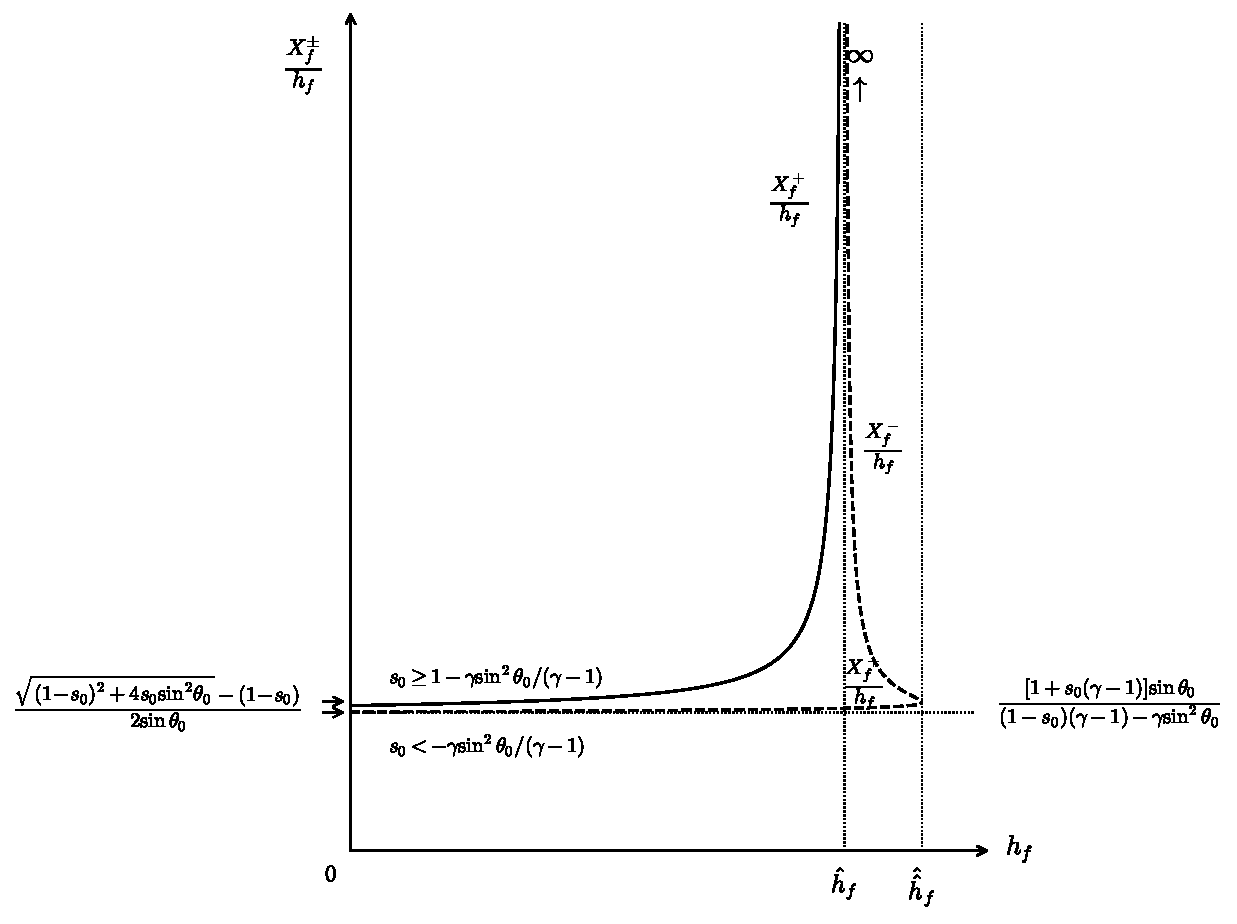
\includegraphics[width=1.0\textwidth]{FShock.pdf}
% \caption{磁流体力学快磁声激波关系.} \label{FShock}
% %\end{center}
% \end{minipage}
% \end{figure}


\section{分工说明}
王玉宝提供了程序、图件,编写了部分LATEX文档;季春瑜提供了部分程序、图件;马新玲编写了部分LATEX文档。

\section{总结和收获}
通过本次作业，我们练习使用python和matlab完成较为复杂科学图片的绘制，尤其练习了在图片上增加字符、公式等辅助理解手段。
另外我们也首次参考科技论文的格式完成了本文件的编写，练习了如何在latex文本中添加链接和引用文献。
上述练习将帮助我们在以后的工作中更方便、高效地展现研究成果。

\section{附件}

% \begin{enumerate}
% \item
% Assign1.tex--本报告 \LaTeX 文件
% \item
% Assign1.pdf--本报告 PDF 输出文件

% \item
% Friedrich.pdf--图~\ref{Friedrich} 的 PDF 图形文件
% \item
% coldp.pdf--图~\ref{ColdPlasma} 的 PDF 图形文件
% \item
 
% FShock.pdf--图~\ref{FShock} 的 PDF 图形文件
% \item
% Code1.txt--文中图~\ref{Friedrich} 所用的python计算和图形绘制程序
% \item
% Code2.txt--文中图~\ref{ColdPlasma} 所用的python计算和图形绘制程序
% \item
% Code3.txt--文中图~\ref{FShock} 所用的matlab计算和图形绘制程序
% \item
% References.bib -- 文献文件
% \end{enumerate}

% 以下两行是中文文献国家标准的格式, 如果安装了这两个格式, 建议使用它们
% \bibliographystyle{gbt7714-author-year}
% \bibliographystyle{gbt7714-numerical}
%

\bibliographystyle{unsrt}
\bibliographystyle{apalike}
\bibliography{References}

% \begin{thebibliography}{1}

% \bibitem{Diver2001}
% Declan~A. Diver.
% \newblock {\em A plasma formulary for physics, technology and astrophysics}.
% \newblock Wiley VCH, 1st edition, 2001.

% \bibitem{Jeffrey1964}
% A.~Jeffrey and T.~Taniuti.
% \newblock {\em Non-Linear Wave Propagation with Applications to Physics and
%  Magnetohydrodynamics}, volume~9 of {\em Mathematics in Science and
%  Engineering - A Series of Monographs and Textbooks}.
% \newblock Academic Press, New York / London, 1964.

% \end{thebibliography}

\end{document}
